\chapter{Introduction}
Humans have deepened their understanding of the world through research, leading to groundbreaking innovations. Research is the foundation of human progress and sets the stage for the future. Such endeavors are considered highly intellectual human activities.
% 人間は研究によってこの世界の理解を深め、この世界にまだないものを生み出すことで、人類の可能性を広げてきました。研究は人類の発展を支えてきた礎であり、まだみぬ未来をより豊かなものにする基盤です。このような、この世にまだない知識を生み出す活動である研究活動は、極めて高度な知的活動と認識されてきました。

Since the beginning of AI research, a key goal has been to develop AI that conducts research. There have been advances in systems that automate scientific judgments \cite{lindsay1993dendral}, infer scientific laws \cite{langley1987scientific}, and autonomously cycle through hypothesis and experimentation \cite{king2004functional}. Recently, with advancements in machine learning, we've seen remarkable successes in using it for scientific discovery \cite{wang2023scientific,xu2021artificial,zhang2023artificial}.
% こうした研究という活動ができる人工知能(AI)を実現することは、AI研究が始まって以来目指されてきました。例えば科学者が行う判断を自動化したシステム \cite{lindsay1993dendral} や、実験データから科学的法則を自動で発見するシステム \cite{langley1987scientific}、自律的に仮説生成と実験のサイクルを回すシステム \cite{king2004functional} などが生み出されました。近年では、機械学習の急速な発展を受けて、機械学習を科学発見に活用することで、重要な科学的発見を上げるような成果も生み出されるまでになりました \cite{wang2023scientific,xu2021artificial,zhang2023artificial}。

On the other hand, the quest to develop a fully autonomous AI that conducts research is still ongoing \cite{zenil2023}. ``Autonomous'' implies the absence of human intervention, prior design, or preparation. I will refer to an AI as being more autonomous if it can conduct research with less human intervention. By ``AI that conducts research,'' I mean a single system that can conduct any research. This includes exploring various fields like history, mathematics, or physics. I label such AI as a ``general artificial researcher.'' The more fields of research a single AI can handle, the more general-purpose I consider that AI to be. 
We emphasize autonomy and generality because it is believed that only when AI possesses these qualities can I say that it's not just a tool for research, but that the AI itself is capable of conducting research. Realizing such a general and autonomous artificial researcher is a significant milestone for humanity.
% 一方で、完全に自律的に自分で研究ができる人工知能がどのようにしたら実現できるのかは依然としてオープンクエスチョンです \cite{Zenil2023}。ここで自律的とは文字通り、人間の介入がないことを意味しています。また、「研究ができる人工知能」とは、現在研究と呼ばれている全ての活動ができる単一の人工知能を意味しています。歴史学であれ数学であれ物理学であれ、任意の研究ができる人工知能であるという意味で、私たちはこれを汎用的な人工研究者と呼んでいます。このような、汎用的で自律的な人工研究者の実現は、人類にとっての大きな目標です。

This paper delves into the concept of a general and autonomous artificial researcher, aiming to set the stage for discussions of possibility for its realization \footnote{
The manuscript is being managed on GitHub \url{https://github.com/t46/research-automation-perspective-paper}, and contributions from everyone to the paper are welcome. The version you are currently reading is a provisional one, and I plan to continue updating it regularly. If you have any suggestions for modifications or find any mistakes, it would be helpful if you could submit a pull request to the repository.
}. 
First, I explore what constitutes research. This helps us to clarify the goal, understand what is required to create the AI, and grasp the implications towards the goal. Next, I briefly review the research fields related to research automation. Viewing these through the lenses of generality and autonomy, I assess the current state of humanity against this goal. Finally, I discuss challenges and suggest a possible first step towards this goal.
% この論文は、この目標の実現へ向けた議論のたたき台を提供すべく、汎用的で自律的な人工研究者について議論します。まず初めに、研究と呼ばれている営みはどのようなものであるかについて議論します。これによって目指すべき目標をより明確にし、研究ができるAIを作るためには何が必要か、それはどのような含意を持つのか、についての示唆を得ることを目指します。次に、研究ができるAIの開発に関連する研究として、研究の自動化に関する研究分野を簡単におさらいします。そして、それらが汎用性と自律性という観点からどのように整理しうるかについて議論し、目標に対する我々人類の現在地を理解することを目指します。最後に、これらの議論を受けて、目標に向けた一歩目としてありうるアプローチや、解決すべき課題について議論します。


% \section{Outline of this Paper}
% The purpose of this perspective paper is to provide a stepping stone towards achieving a general and autonomous artificial researcher as quickly as possible. It aims to offer information that enables all those pursuing this goal to focus on essential issues, avoid reinventing the wheel, and maximize their own potential. This is because I believe that enabling the full potential of brilliant researchers worldwide is the most crucial for accomplishing this objective.

% To achieve the purpose of this paper, I will discuss three key points in chapters 2, 3, and 4, respectively: What is the goal, where are I currently standing, and what to do to achieve the goal. First, in chapter 2, I will delve into the discussion of ``What is the goal'' to make the common objective clearer for everyone involved. By doing so, researchers and engineers all over the world are able to devise methods to achieve this goal even before looking at our proposals in this paper. Furthermore, this discussion aims to clarify the limits and possibilities of a general and autonomous artificial researcher. Specifically, I will thoroughly discuss ``What is research?'' as it is essential to understand what a ``general'' artificial researcher entails. Starting with the definition of research, I will examine the functions that various research activities serve and discuss the implications of achieving this through artificial intelligence.

% Next, in chapter 3, I will discuss ``Where are I currently standing'' to work towards a state where researchers pursuing research automation no longer need to gather preliminary information on their own. To that end I will briefly introduce some examples of past initiatives related to the automation of research.
% accomplish this, I conduct a literature review on research automation. I will organize studies related to research automation, discuss their relationships and current status. In this survey, I will strive for as much comprehensiveness as possible, including anything relevant to research automation, no matter how superficial, as I believe that once researchers become aware of the research area, they can delve deeper into specific aspects on their own. Additionally, I observed a lack of information sharing among various individual efforts related to research automation, and by addressing these diverse approaches in a unified manner within one paper, I aim to promote information exchange between different fields.

% In chapter 4, I will discuss the challenges for the goal and some ideas as am initial step towards the goal. Building upon the clarity of the goal from chapter 2 and the understanding of the current state from chapter 3, I will discuss how to bridge the gaps between them. I will also explore the directions and specific approaches for research and development, suggesting the policies and avenues that may be most effective.

% Moreover, this paper is licensed under the OO license, so feel free to make any modifications you see fit. If you wish to follow the main structure, you can fork the repository, or if you have a different approach in mind, you can create an entirely new project.

% I hope this paper can contribute in some way to the advancement of automation in research. Thank you.


% Additionally, this paper is intended to be updated on an ongoing basis. If you find points that you think are lacking or inaccuracies in understanding, please send a Pull Request on GitHub. Based on that, I will revise the content of the paper as needed.

% \section{Others}

% The purpose of this perspective paper is to discuss the possibility of automating this activity of research, that is, the realization of intelligent agents capable of conducting research autonomously. After summarizing attempts at research automation so far, I intend to present our personal perspective on promising ideas, necessary elements, and ways to proceed in order to create artificial researchers. In particular, this paper is aimed at machine learning researchers and developers, with the goal of increasing the number of colleagues aiming for research automation by providing concrete possible actions.

% One thing to note here is that our aim is not to automate or substitute the current research tasks, but to create intelligent agents capable of conducting research. In other words, as long as it is research, automated research may at first glance seem to be far removed from the current research activities. This is because the current research activity may not necessarily be the absolute optimal form in light of its purpose. 

% First, the optimal form is always influenced by the context of history. Of course, the optimum in the era when letterpress printing was mainstream is different from the optimum in the era when the Internet became infrastructure. Research itself has changed its form over time, and the optimal form of research in the present or future can naturally change. Moreover, as Nielsen and Qiu say \cite{nielsen}, it is believed that I have only explored a very limited range regarding the practice of research. The establishment of current research practices is a very recent event in human history, and I may not yet have arrived at the optimum way of intellectual production. Furthermore, current research assumes that humans are the main creators of knowledge. This naturally imposes human cognitive constraints, which may significantly limit the range of activities that can be conducted for knowledge production. 

% Therefore, instead of thinking about how to automate and streamline current tasks, I discuss the possibility of realizing intelligent agents that can autonomously perform the fundamental and core elements of research activity in a more optimal form, and what is necessary for this.

% \textcolor{red}{TODO: Add lots of high-level illustration}

% \section{TODO}

% To reiterate, \textbf{the proposition put forward in this paper is to strive for the realization of general and autonomous artificial researcher}. Autonomy refers to the level of human intervention and design involved. For instance, a system that requires humans to explicitly provide a set of hypotheses has lower autonomy compared to one that allows the machine to discover them on its own.  Generality refers to how many research fields a single automated research system can handle. For example, a system capable of conducting research in both physics and history is more general compared to a system limited to either one.

% While it might be easier to grasp what a more autonomous system is, the challenge lies in defining what a general artificial researcher is. This is because I need to comprehend what it means for a system to be capable of both physics and history research, for example. Therefore, to create a general artificial researcher, it seems necessary to first define what research itself is. By discussing what constitutes research and what is required to conduct it, I may uncover the abilities that the system must possess. Hence, the following sections will explore the fundamental nature of research. After discussing autonomy a bit below, I will discuss what research is all about.

% \begin{figure}[htb]
%     \centering
%     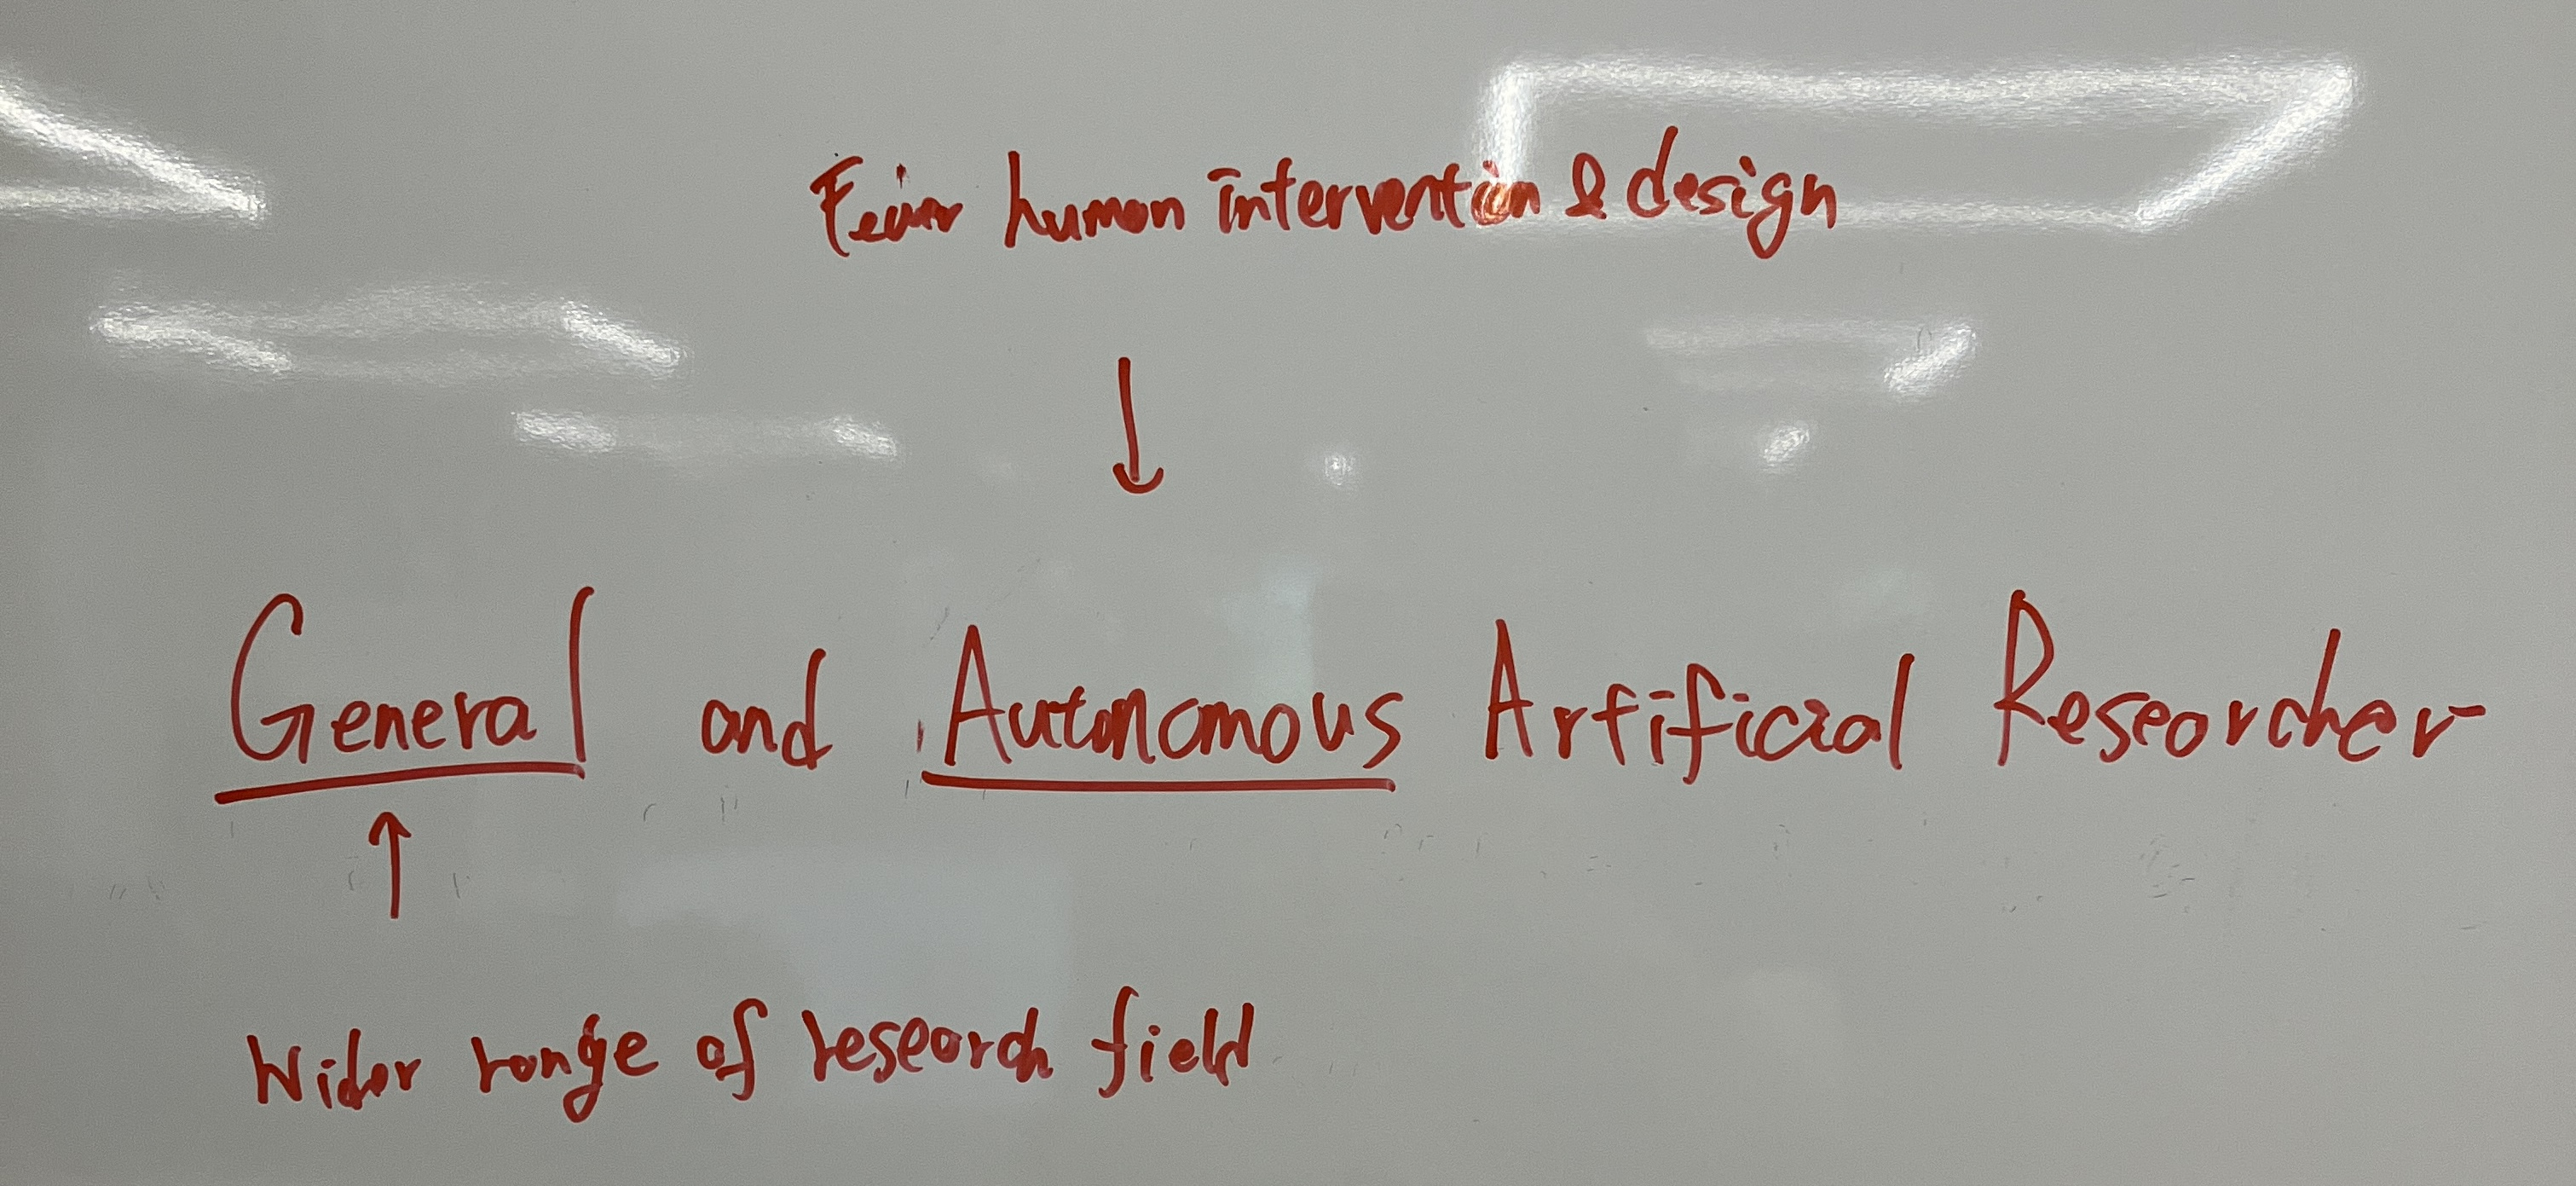
\includegraphics[width=\linewidth]{figs/goal.jpg}
%     \caption{General and Autonomous Artificial Researcher}
%     \label{fig:goal}
% \end{figure}

% \subsubsection{Level of Autonomy}
% What I are aiming for is an artificial intelligence that can conduct research completely autonomously. Therefore, the ultimate aim is to minimize predetermined modules or algorithms decided by humans and create an end-to-end system. With that in mind, I would like to express our opinion on how much autonomy should be pursued.

% Firstly, autonomy ultimately boils down to the question of how much is taken for granted. The more predetermined elements there are, the lower the autonomy, and the fewer predetermined elements there are, the higher the autonomy. In this sense, autonomy is continuous and incremental.

% The highest level of autonomy in pursuing the realization of an artificial researcher is a state where the system invents and conducts research without even assuming its purpose as research. This means not instructing the system to conduct research, not teaching what research is beforehand, but enabling the acquisition and execution of research. Humans can be considered researchers with this level of autonomy at least at the species level. This is because while humans are probably not designed as systems dedicated solely to research, they have progressively invented research throughout history. Of course, such a level of autonomy is not achievable without any assumptions, so if one aims for this level of autonomy, it is necessary to prepare an environment that induces the acquisition of research and design some form of inductive bias. What I are referring to here is a system with autonomy in the sense that research is acquired as a result of computational processing indirectly related to knowledge production and the necessary conditions for it.

% However, demanding such a level of autonomy may be somewhat excessive when it comes to pursuing an autonomous artificial researcher. Therefore, it seems reasonable to assume research as a design requirement. Since research is assumed to be the purpose, some form of information about what knowledge is must be provided. Here, I can classify it into two categories.

% The first is implicitly providing information about what research is. This involves allowing the system to acquire the concept of research on its own based on existing knowledge and data about the process of research. The history of machine learning research has shown the power of this end-to-end direction in creating strong intelligent systems. In that sense, this direction can be considered one of the directions to pursue.

% The second is explicitly providing information about what research is. This involves providing only the necessary information about the conditions related to research and aiming for their fulfillment. It does not mean explicitly instructing how to construct questions or specific means to justify beliefs. Instead, it only provides information about what needs to be done, and the system must acquire and execute them on its own. This is autonomy in the sense that one must acquire the methods oneself and execute them. I believe that if I provide information at this level, it can be considered a system capable of conducting research autonomously. On the other hand, I think that research achieved by hard-coding the each single process within the research is not autonomous. It is expected to be quite challenging to aim for the first one   directly. Therefore, I believe it is better to aim for the third level of autonomy. 

% A particularly serious part of building an autonomous system is the question of what to do with the initial values. This is because some input must be given as a given, and the question is to what extent this information can be given by a human being and still be called autonomous. This will be discussed again in this paper.